\documentclass[11pt]{article}
\usepackage[shortlabels]{enumitem}
\usepackage[margin=1in,headheight=15pt]{geometry}   % Adjusted headheight
\usepackage{amsmath}
\usepackage{fancyhdr}
\usepackage{graphicx}
\usepackage{cancel}
\usepackage{amsfonts}
\usepackage{setspace}

% Set up fancy header/footer
\pagestyle{fancy}
\fancyhead[LO,L]{Jimmy Chen}
\fancyhead[CO,C]{CSCI 2500 - Computer Organization}
\fancyhead[RO,R]{November 13, 2023}
\fancyfoot[LO,L]{}
\fancyfoot[CO,C]{\thepage}
\fancyfoot[RO,R]{}
\renewcommand{\headrulewidth}{0.4pt}
\renewcommand{\footrulewidth}{0.4pt}
\graphicspath{ {./images/} }
\onehalfspacing

\begin{document}
\section{Homework 3}

% BOOLEAN ALGEBRA QUESTIONS
\subsection{Boolean Algebra}
\begin{enumerate}
    % Question 1
    \item Simplify the following expressions using Boolean algebraic laws. Give each step of your simplification and denote which laws you’re using for each step. Do not skip or combine steps!
    \begin{enumerate}[(a)]
        % =========Question 1a=========
        \item  $A * (\overline{A}+B*B) + (\overline{B+A}) * (\overline{A} + B)$\\
        \textbf{Work:}
        \begin{center}
            $A * (\overline{A} + B) + (\overline{B + A}) * (\overline{A} + B)$ // Idempotent law\\
            $A * B + (\overline{B + A}) * (\overline{A} + B)$ // Redundancy law\\
            $A * B + \overline{B} * \overline{A} * (\overline{A} + B)$ // Demorgan's law\\
            \fbox{\begin{minipage}{15em}
                \begin{center}
                \textbf{Answer: $A * B + \overline{B} * \overline{A}$}
                \end{center}
            \end{minipage}}
        \end{center} 
        % =========Question 1b=========
        \item $\overline{C * B} + ( A * B * C) + \overline{A + B + \overline{B}}$\\
        \textbf{Work:}
        \begin{center}
            $\overline{C} + \overline{B} + (A * B * C) + \overline{A + C + \overline{B}}$ // Demorgan's law\\
            $\overline{C} + \overline{B} + (A * B * C) + \overline{A} * \overline{C} * B$ // Involution Law\\
            $\overline{C} + \overline{B} + A * B * C$ // Absorption Law\\
            $\overline{C} + \overline{B} + A * B$ // Absorption Law\\
            $\overline{C} + \overline{B} + A$ // Absorption Law\\
            \fbox{\begin{minipage}{15em}
                \begin{center}
                \textbf{Answer: $\overline{C} + \overline{B} + A$}
                \end{center}
            \end{minipage}}
        \end{center}
        % =========Question 1c=========
        \item $(A + B) * (\overline{A} + C) * (\overline{C} + B)$ \\
        \textbf{Work:}
        \begin{center}
            $(\overline{A} + C) * (\overline{C} + B) * A + (\overline{A} + C) * (\overline{C} + B) * B$ // Distributive Law\\
            $(\overline{C} + B) * A * \overline{A} + (\overline{C} + B) * A * C + (\overline{A} + C) * (\overline{C} + B) * B$ // Distributive Law\\
            $0 + (\overline{C} + B) * A * C + (\overline{A} + C) * (\overline{C} + B) * B$ // Complement Law\\
            $(\overline{C} + B) * A * C + (\overline{A} + C) * (\overline{C} + B) * B$ // Identity Law\\
            $A * A * \overline{C} + A * C * B + (\overline{A} + C) * (\overline{C} + B) * B$ // Distributive Law\\
            $0 + A * C * B + (\overline{A} + C) * (\overline{C} + B) * B$ // Complement Law\\
            $A * C * B + (\overline{A} + C) * (\overline{C} + B) * B$ // Identity Law\\
            $A * C * B + B * \overline{A} * \overline{C} + B * \overline{A} * B + (\overline{C} + B) * B * C$ // Distributive Law\\
            $A * C * B + B * \overline{A} + (\overline{C} + B) * B * C$ // Absorption Law\\
            $B * (A * C + \overline{A}) + (\overline{C} + B) * B * C$ // Distributive Law\\
            $B * (C + \overline{A}) + (\overline{C} + B) * B * C$ // Absorption Law\\
            $B * C + B * \overline{A} + (\overline{C} + B) * B * C$ // Distributive Law\\
            $B * C + B * \overline{A}$ // Absorption Law\\
            \fbox{\begin{minipage}{15em}
                \begin{center}
                \textbf{Answer: $B * C + B * \overline{A}$}
                \end{center}
            \end{minipage}}
        \end{center}
    \end{enumerate}
    
    % Question 2
    \item Find all solutions of the following Boolean equations without using the truth tables:
    \begin{enumerate}[(a)]
        % =========Question 2a=========
        \item $(\overline{A} + C) * (\overline{B} + D + A) * (D + A * \overline{C}) * (\overline{D} + A) = 1$\\
        \textbf{Work:}\\
            $ (\overline{A} * \overline{B} + \overline{A} * D + \overline{A} * A + \overline{B} * C + C * D + C * A) * (D + A * \overline{C}) * (\overline{D} + A) = 1$ //Distributive\\
            $ (\overline{A} * \overline{B} + \overline{A} * D + 0 + \overline{B} * C + C * D + C * A) * (D + A * \overline{C}) * (\overline{D} + A) = 1$ //Complement\\
            $ (\overline{A} * \overline{B} + \overline{A} * D + \overline{B} * C + C * D + C * A) * (D * \overline{D} + \overline{C} * A \overline{D} + \overline{C} * A) = 1$\\
            $ (\overline{A} * \overline{B} + \overline{A} * D + \overline{B} * C + C * D + C * A) * (0 + A * D + \overline{C} * A * \overline{D} + A * \overline{C} * A) = 1$\\
            $ (\overline{A} * \overline{B} + \overline{A} * D + \overline{B} * C + C * D + C * A) * (D * A + A * \overline{C} * \overline{D} + A * \overline{C} * A) = 1$ //Identity\\
            $ (\overline{A} * \overline{B} + \overline{A} * D + \overline{B} * C + C * D + C * A) * (D * A + A * \overline{C} * \overline{D} + A * \overline{C}) = 1$ //Idempotent\\ 
            $ (\overline{A} * \overline{B} + \overline{A} * D + \overline{B} * C + C * D + C * A) * (D * A + A * \overline{C} * (\overline{D} + 1)) = 1$ //Distributive\\
            $ (\overline{A} * \overline{B} +  \overline{B} * C + C * D + C * A) * (D * A + A * \overline{C}) = 1$ //Identity Law\\
            $ (\overline{A} * \overline{B} * D * A + \overline{A} * D * D * A + C * \overline{B} * D * A + C * D * D * A + C * A * D * A) + \overline{A} * \overline{B} * \overline{C} * A + \overline{A} * D * \overline{C} * A + C * \overline{B} * \overline{C} * A + C * D * \overline{C} * A + C * A * \overline{C} * A = 1$ //Distributive\\
            $ (0 + 0 + C * \overline{B} * D * A + C * D * D * A + C * A * D * A) + 0 + 0 + C * \overline{B} * \overline{C} * A + C * D * \overline{C} * A + C * A * \overline{C} * A = 1$\\
            $ (0 + 0 + C * \overline{B} * D * A + C * D * D * A + C * A * D * A) + 0 + 0 + 0 + 0 + 0 = 1$ //Complement\\
            $ C * \overline{B} * D * A + C * D * D * A + C * A * D * A = 1$ //Identity Law\\
            $ C * \overline{B} * D * A + A * C * D + C * A * D= 1$ //Idempotent Law\\
            $ C * \overline{B} * D * A + A * C * D = 1$ //Idempotent Law\\
            $ (\overline{B} + 1) * A * C * D = 1$ //Distributive Law\\
            $ A * C * D = 1$ //Identity Law
            \begin{center}
                \fbox{\begin{minipage}{15em}
                    \begin{center}
                    \textbf{Answer: $A = 1, C = 1, D = 1$}\\
                    \textit{B can be anything}
                    \end{center}
                \end{minipage}}
            \end{center}
        % =========Question 2b=========
        \item $(((\overline{K} * L * N) * (L * M)) + ((\overline{K} + L + N) * (K * \overline{L} * \overline{M}))) * (\overline{K} + \overline{N}) = 1$\\
        \textbf{Work:}\\
            $(((\overline{K} * L * L * N) + \overline{K} * L * N * M) + ((\overline{K} * K * \overline{L} * \overline{M} + L * K * \overline{L} * \overline{M} + N * K * \overline{L} * \overline{M})))*(\overline{K}+\overline{N}) = 1$ //Distributive Law\\
            $(((\overline{K} * L * L * N) + \overline{K} * L * N * M) + ((0 + 0 + K * N * \overline{L} * \overline{M}))) * (\overline{K}+ \overline{N}) = 1$ //Complement\\  
            $(((\overline{K} * L * L * N) + \overline{K} * L * N * M) + ((K * N * \overline{L} * \overline{M}))) * (\overline{K} + \overline{N}) = 1$ //Identity Law\\
            $(\overline{K}* L * L * N + \overline{K} * L * N * M + N * K * \overline{L} * \overline{M}) * (\overline{K} + \overline{N}) = 1$ //Commutative Law\\
            $(\overline{K}* L * L * N + \overline{K} * L * N * M * \overline{K} + K * N * \overline{L} * \overline{M} * \overline{K}) + \overline{K} * L * L * N * \overline{N} + \overline{K} * L * N * M * \overline{N} + N * K * \overline{L} * \overline{M} * \overline{N} = 1$ //Distributive Law\\
            $(\overline{K}* L * L * N + \overline{K} * L * N * M * \overline{K} + 0) + 0 + 0 + 0= 1$ //Complement Law\\
            $(\overline{K} * L * N + \overline{K} * L * N * M + 0) + 0 + 0 + 0 = 1$ //Idempotent Law\\
            $(\overline{K} * L * N + \overline{K} * L * N * M) = 1$ //Identity Law\\
            $(\overline{K} * L * N(1 + M)) = 1$ //Distributive Law\\
            $\overline{K} * L * N = 1$ //Identity Law
            \begin{center}
                \fbox{\begin{minipage}{15em}
                    \begin{center}
                    \textbf{Answer: $K = 0, L = 1, N = 1$}\\
                    \textit{M can be anything}
                    \end{center}
                \end{minipage}}
            \end{center}
    \end{enumerate}

    % Question 3
    \item Simplify the following expression by first constructing a truth table, using that truth table to
    construct a K-map, and then using that K-map to simplify.\\
    $Q = \overline{X} * \overline{Y} * Z + X * Y * \overline{Z} + \overline{X} + Y * \overline{Z} + X * \overline{Y} * \overline{Z}$\\
    \textbf{Work:}
    \begin{center}
        \textbf{Truth Table:}\\
        \begin{tabular}{c c c | c}\\
            X & Y & Z & Q \\
        \hline
            0 & 0 & 0 & 0 \\
            0 & 0 & 1 & 0 \\
            0 & 1 & 0 & 1 \\
            0 & 1 & 1 & 1 \\
            1 & 0 & 0 & 0 \\
            1 & 0 & 1 & 0 \\
            1 & 1 & 0 & 0 \\
            1 & 1 & 1 & 1 \\
        \end{tabular}\\ [0.25in]

        \textbf{K-Map:}\\[0.15in]
        \begin{tabular}{c | c | c | c | c |}
            \textbf{X\textbackslash YZ} & \textbf{00} & \textbf{01} & \textbf{11} & \textbf{10}\\
            \hline
            \textbf{0} & 0 & 1 & 0 & 1\\
            \hline
            \textbf{1} & 0 & 0 & 1 & 0\\
            \hline
        \end{tabular}\\[0.25in]
        
        \fbox{\begin{minipage}{20em}
            \begin{center}
                \textbf{Simplified Answer:} $Q = \overline{X} * Z + X * \overline{Y} * \overline{Z}$\\
            \end{center}
        \end{minipage}}\\[0.25in]
        
    \end{center}
\end{enumerate}

\subsection{Logical Circuits}
\begin{enumerate}
    \setcounter{enumi}{3}
    % Question 4
    \item Convert the following truth table into its sum of products representation:\\
    \begin{tabular}{c c c | c}\\
            A & B & C & Output \\
        \hline
            0 & 0 & 0 & 1 \\
            0 & 0 & 1 & 1 \\
            0 & 1 & 0 & 0 \\
            0 & 1 & 1 & 0 \\
            1 & 0 & 0 & 1 \\
            1 & 0 & 1 & 0 \\
            1 & 1 & 0 & 1 \\
            1 & 1 & 1 & 0 \\
    \end{tabular}\\
    \textbf{Work:}
    \begin{center}
        \begin{tabular}{c c c | c}
            0 & 0 & 0 & 1  = $\overline{A} * \overline{B} * \overline{C}$\\
        \end{tabular}\\
        \begin{tabular}{c c c | c}\\
            0 & 1 & 0 & 1  = $\overline{A} * B * \overline{C}$\\
        \end{tabular}\\
        \begin{tabular}{c c c | c}\\
            0 & 1 & 1 & 1  = $\overline{A} * B * C$\\
        \end{tabular}\\
        \begin{tabular}{c c c | c}\\
            1 & 1 & 1 & 1  = $A * B * C$\\
        \end{tabular}\\[0.15in]
        \fbox{\begin{minipage}{30em}
            \begin{center}
            $\overline{A} * \overline{B} * \overline{C} + \overline{A} * B * \overline{C} + \overline{A} * B * C + A * B * C$\\
            \textbf{Simplified Answer: $\overline{A} * \overline{C} + B * C$}
        \end{center}
        \end{minipage}}
    \end{center}

    % Question 5
    \item Draw a logical circuit diagram that represents the above sum of products expression using OpenCircuits (https://opencircuits.io/). Clearly label all inputs/outputs and all
    components. Make sure you connect appropriate input components (e.g., buttons, switches, clocks, etc.) and output components (e.g., LEDs, displays, etc.) to facilitate testing of
    your circuit.Download your diagram using OpenCircuits' “Download” feature, rename it to
    hw3\_SOP.circuit, and submit on Submitty along with your hw3.pdf file.\\[0.25in]
    \textbf{Answer: The Circuit below was uploaded to Submitty}\\
    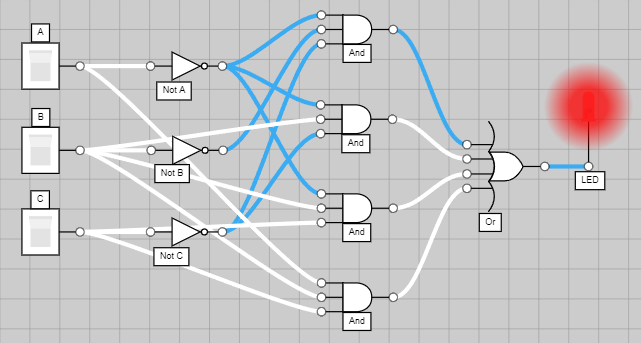
\includegraphics[scale=0.6]{0_0_0}
    % Question 6
    \item Test you circuit by supplying appropriate inputs and observing the expected values of the
    output. Explain why your set of tests is sufficient to prove that your logical circuit does in
    fact implement the required Boolean function. For each test, provide a picture (snapshot) of
    your circuit. Insert all such pictures in the hw3.pdf PDF file. You can download pictures
    (PNG, JPEG, or PDF) of your circuit diagram using OpenCircuits' “Export Image” feature.\\[0.25in]
    \textbf{Answer:}\\
        Below are the images of the circuit being tested. There are a total of 8 test photos, and they cover all the possible cases.\\[0.55in]
    \textbf{Images:}\\
        Case 1: A = 0, B = 0, C = 0; the output is 1, which corresponds to the boolean function\\
        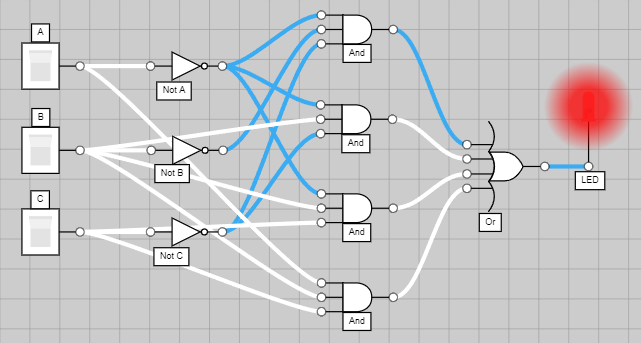
\includegraphics[scale=0.6]{0_0_0}\\[0.25in]
        Case 2: A = 0, B = 1, C = 0; the output is 1, which corresponds to the boolean function\\
        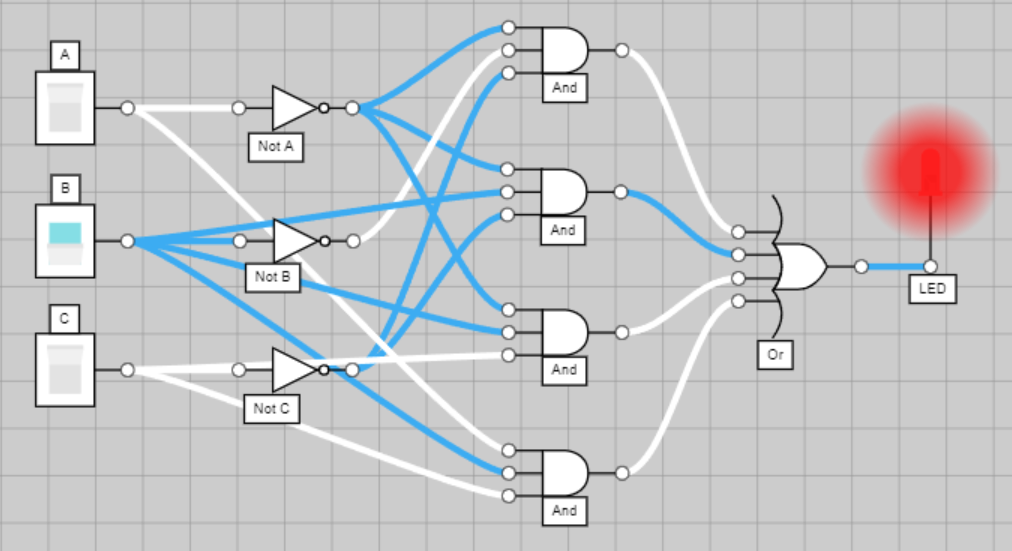
\includegraphics[scale=0.38]{0_1_0}\\[0.25in]
        Case 3: A = 0, B = 1, C = 1; the output is 1, which corresponds to the boolean function\\
        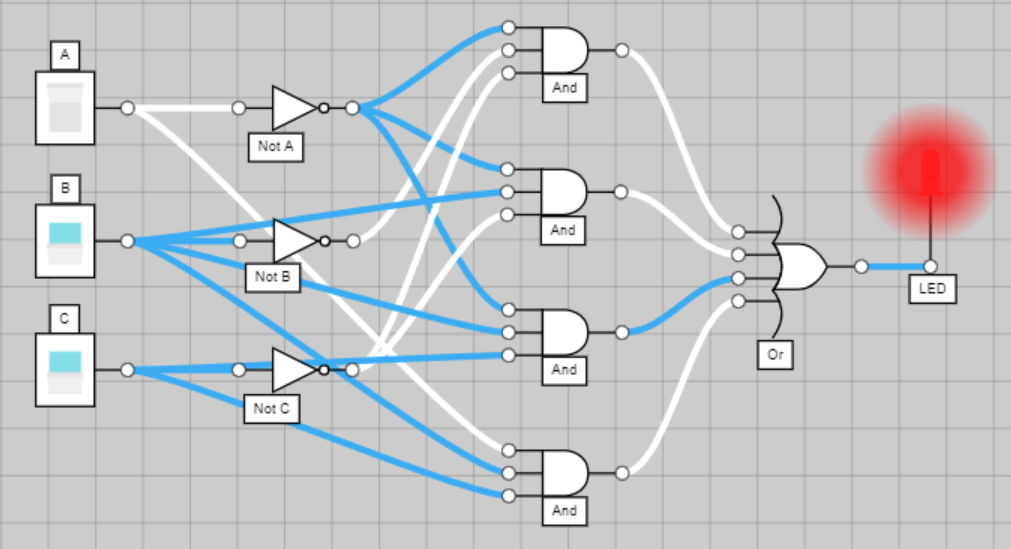
\includegraphics[scale=0.38]{0_1_1}\\[0.25in]
        Case 4: A = 1, B = 1, C = 1; the output is 1, which corresponds to the boolean function\\
        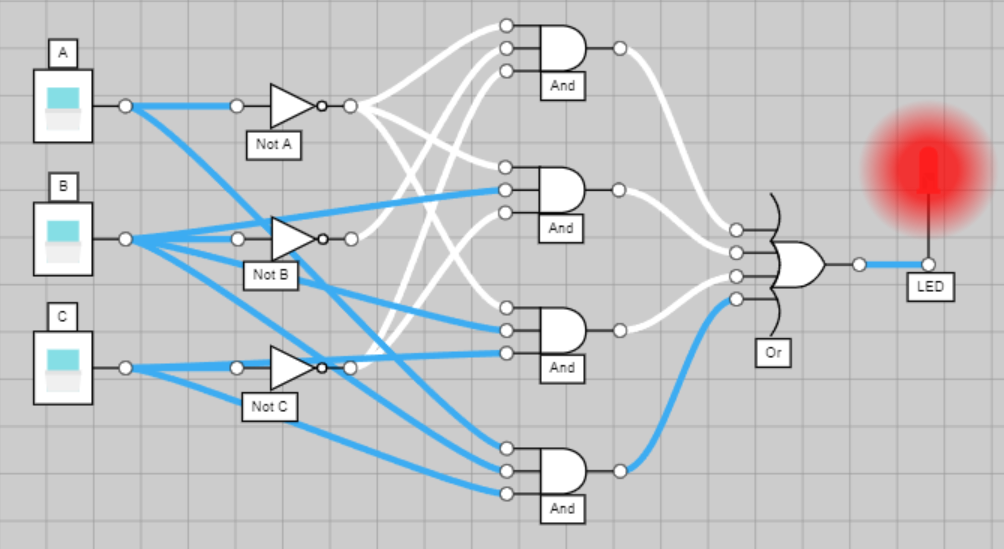
\includegraphics[scale=0.38]{1_1_1}\\[0.25in]
        Case 5: A = 1, B = 0, C = 1; the output is 0, which corresponds to the boolean function\\   
        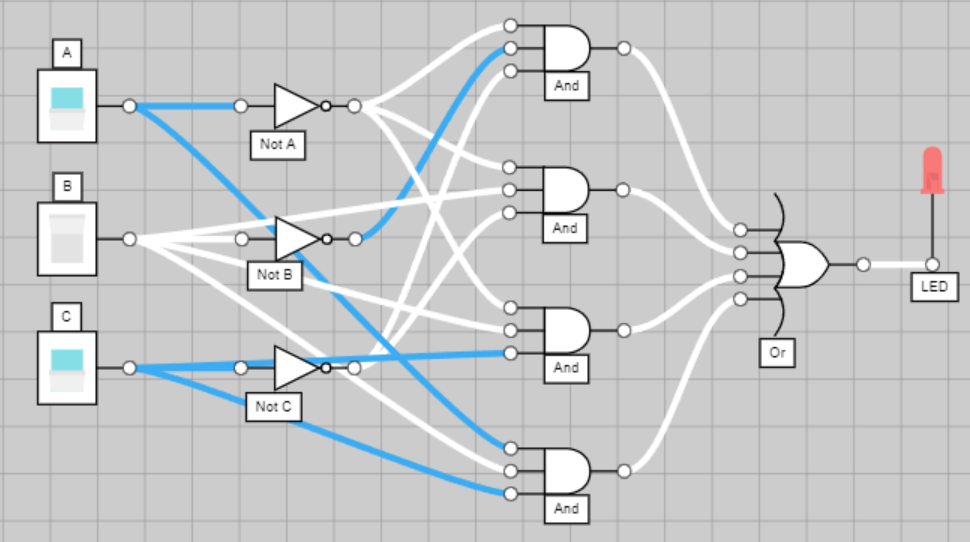
\includegraphics[scale=0.395]{1_0_1}\\[0.25in]
        Case 6: A = 1, B = 0, C = 0; the output is 0, which corresponds to the boolean function\\
        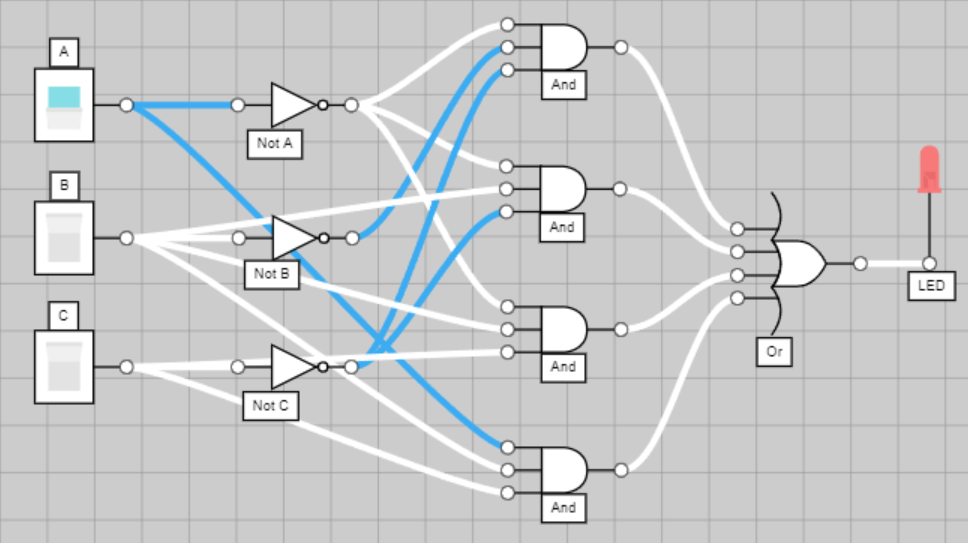
\includegraphics[scale=0.395]{1_0_0}\\[0.25in]
        Case 7: A = 0, B = 0, C = 1; the output is 0, which corresponds to the boolean function\\
        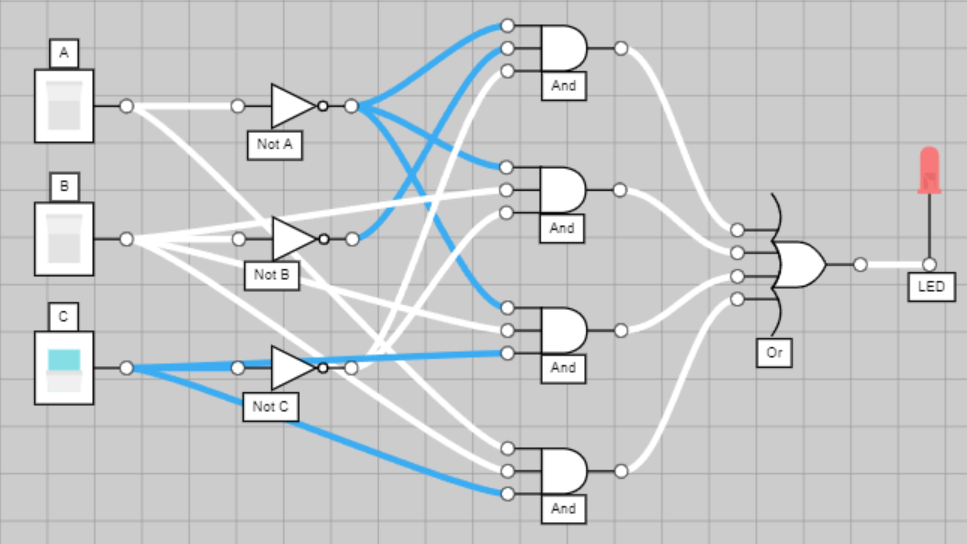
\includegraphics[scale=0.395]{0_0_1}\\[0.25in]
        Case 8: A = 1, B = 1, C = 0; the output is 0, which corresponds to the boolean function\\
        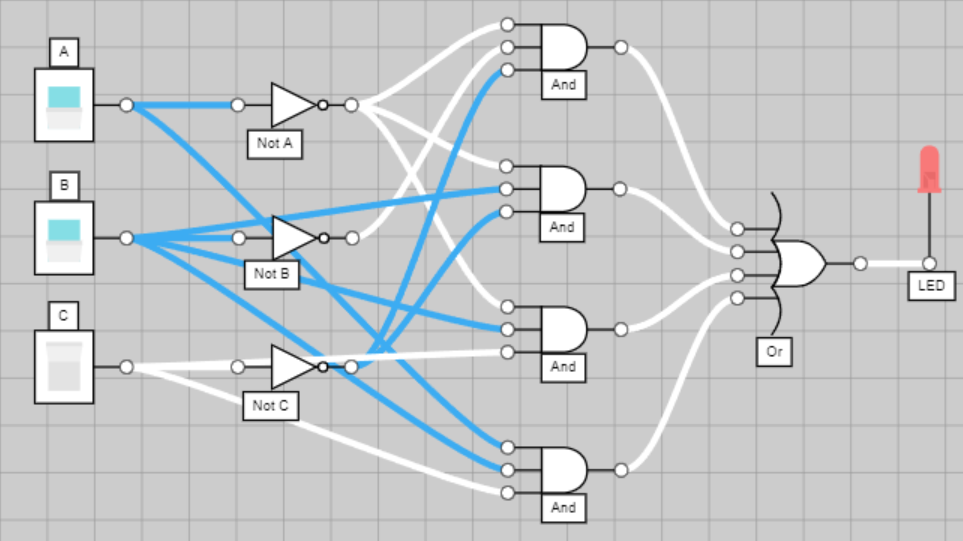
\includegraphics[scale=0.4]{1_1_0}
    % Question 7
    \item Given inputs A and B, show that NOR \{$(\overline{A + B})$\} is functionally complete by giving logical
    circuits equivalent to AND \{$(A * B)$\}, OR \{$(A + B)$\}, and NOT \{$(\overline{A})$\} using only NOR gates in their construction.\\[0.25in]
    \textbf{Images:}\\
    NOR to create: AND Gate\\
    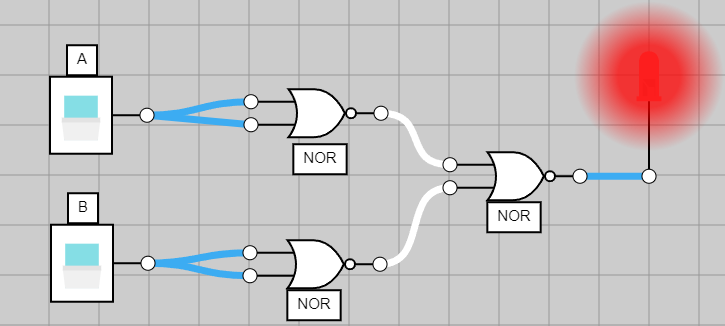
\includegraphics[scale=0.47]{and}\\[0.25in]
    NOR to create: OR Gate\\
    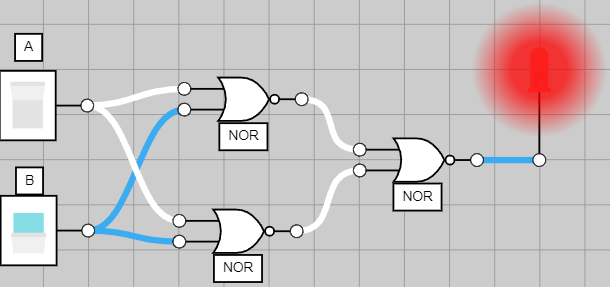
\includegraphics[scale=0.55]{or}\\[0.25in]
    NOR to create: NOT Gate\\
    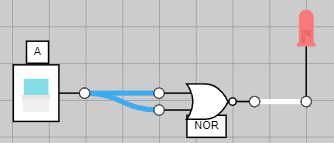
\includegraphics[scale=1]{not}
\end{enumerate}

\subsection{Numerical Conversions and Arithmetic}
\begin{enumerate}
    \setcounter{enumi}{7}
    % Question 8
    \item For each of the following numbers, convert them to their closest single precision IEEE 754
    floating point representation. First, denote the binary values of the sign, fraction, and exponent. Then provide a 32-bit hexadecimal value. Show your steps.\\
    % =========Question 8a=========
    a. $50.4375$\\
    \textbf{Work:}
    \begin{center}
        Sign: $0$\\
        Exp: $5 + 127 = 132 = 10000100$\\
        Mantissa: $110010.0111 = 1.100100111 * 2^5$\\
        \fbox{\begin{minipage}{23em}
            \begin{center}
            \textbf{Answer: $0\ 10000100\ 10010011100000000000000$}
            \end{center}
        \end{minipage}}
    \end{center}
    % =========Question 8b=========
    b. $0.0$\\
    \textbf{Work:}
    \begin{center}
        Sign: $0$\\
        Mantissa: $0$\\
        \fbox{\begin{minipage}{23em}
            \begin{center}
            \textbf{Answer: $0\ 00000000\ 00000000000000000000000$}
            \end{center}
        \end{minipage}}
    \end{center}
    % =========Question 8c=========
    c. \textit{$-Infinity$}\\
    \textbf{Work:}
    \begin{center}
        Sign: $1$ \textit{// Since it's negative}\\
        Exp: $1$ \textit{// All 1s - which in binary is 11111111}\\
        Mantissa: $0$\\
        \fbox{\begin{minipage}{23em}
            \begin{center}
            \textbf{Answer: $1\ 11111111\ 00000000000000000000000$}
            \end{center}
        \end{minipage}}
    \end{center}
    % =========Question 8d=========
    d. $1.0000001$
    \textbf{Work:}
    \begin{center}
        Sign: $0$ \textit{// Since it's positive}\\
        Exp: $01111111 = 127$\\
        Mantissa: $1.0000001 = 1.0000001 * 2^0$\\
        Normalized: $00000000000000000000001$
        \fbox{\begin{minipage}{23em}
            \begin{center}
            \textbf{Answer: $0\ 01111111\ 00000000000000000000001$}
            \end{center}
        \end{minipage}}
    \end{center}
    %Question 9
    \item For each of the following hexadecimal values, convert them from single precision IEEE 754
    floating point representation to decimal rational numbers. You may leave large powers of
    two in the exponential form, and you may express your answer as a ratio (e.g., $-\frac{5}{8}, \frac{1}{2^{64}}$). \\
    Show your steps.\\
    % =========Question 9a=========
    a. $0xc349a000\\$
    \textbf{Work:}
    \begin{center}
        In Binary Form: $1100 0011 0100 1001 1010 0000 0000 0000$\\
        Sign: $1$ \textit{// Since it's negative}\\
        Exp: $10000110 = 134 = 2^1 + 2^2 + 2^7$\\
        The rest of the bits are the mantissa: $1001 1010 0000 0000 0000 = 2^{-1} + 2^{-4} + 2^{-7} + 2^{-8} + 2^{-10} = 589/1024$\\
        Converting: $(-1^1) * (1 + 589/1024) * 2^{134-127} = -(1613/8)$\\
        \fbox{\begin{minipage}{15em}
            \begin{center}
            \textbf{Answer: $-(1613/8)$}
            \end{center}
        \end{minipage}}
    \end{center}

    % =========Question 9b=========
    b. $0xffe00001\\$
    \textbf{Work:}
    \begin{center}
        In Binary Form: $1111 1111 1110 0000 0000 0000 0000 0001$\\
        Sign: $1$ \textit{// Since it's negative}\\
        Exp: $11111111 = 255 = 2^0 + 2^1 + 2^2 + 2^3 + 2^4 + 2^5 + 2^6 + 2^7$\\
        The rest of the bits are the mantissa: $110 0000 0000 0000 0000 0001 = 2^{-1} + 2^{-2} + 2^{-23} = 6291457 / 2^{23}$
        Converting: $(-1)^1 * (1 + 6291457 / 2^{23}) * 2^{255-127} = -(6291459/2^{104})$\\
        \fbox{\begin{minipage}{15em}
            \begin{center}
            \textbf{Answer: $-(6291459/2^{104})$}
            \end{center}
        \end{minipage}}
    \end{center}

    % =========Question 9c=========
    c. $0x80000000\\$
    \textbf{Work:}
    \begin{center}
        In Binary Form: $1000 0000 0000 0000 0000 0000 0000 0000$\\
        Sign: $1$ \textit{// Since it's negative}\\
        Exp: $00000000 = 0$\\
        The rest of the bits are the mantissa: $000 0000 0000 0000 0000 0000 = 0$\\
        Converting: $(-1)^1 * (1 + 0) * 2^{0-127}$\\
        \fbox{\begin{minipage}{15em}
            \begin{center}
            \textbf{Answer: $-(1/2^{127})$}
            \end{center}
        \end{minipage}}
    \end{center}

    % =========Question 9d=========
    d. $0x00400000$\\
    \textbf{Work:}
    \begin{center}
        In Binary Form: $0000 0000 0100 0000 0000 0000 0000 0000$\\
        Sign: $0$ \textit{// Since it's positive}\\
        Exp: $00000000 = 0$\\
        The rest of the bits are the mantissa: $100 0000 0000 0000 0000 0000 = 2^{-1} = 1/2$\\
        Converting: $(-1)^0 * (1 + 1/2) * 2^{0-127}$\\
        \fbox{\begin{minipage}{15em}
            \begin{center}
            \textbf{Answer: $3/2^{128}$}
            \end{center}
        \end{minipage}}
    \end{center}
    
    % Question 10
    \item Give a reason why we use 2's complement representations for negative numbers in computer
    arithmetic. Give an example of its usage.\\
    \textbf{Answer:}
    \begin{center}
        The 2's complement representation is favored in computer arithmetic for negative numbers because it makes the addition and subtraction of positive and negative numbers easier. 
        This method enables the utilization of the same circuitry for both types of numbers, simplifying hardware implementation and boosting efficiency. 
        Consequently, a single set of instructions suffices for performing arithmetic operations, whether they involve unsigned or signed numbers.

        An example would be if we take the 8-bit bumbers 10 (00001010 in binary) and -6 (11111010 in binary, two's complement) and add them together, we get 4 (00000100 in binary). This is because 10 + (-6) = 4.
        Doing this, there is no special handling for negatives.\\
    \end{center}
\end{enumerate}
\end{document}